% =====================================================================
%  When a Tie Is a Ceiling
%  Tie-saturated rank evaluation in learned prioritization for
%  post-quantum migration.
%
%  Every number in this manuscript is regenerated from the JSON
%  artifacts in paper/analysis/ by the scripts in scripts/paper_*.py
%  at the audited commit. Nothing here is estimated.
% =====================================================================
\documentclass[journal,10pt]{IEEEtran}

\usepackage{amsmath,amssymb,amsthm}
\usepackage{graphicx}
\usepackage{booktabs}
\usepackage{multirow}
\usepackage{array}
\usepackage{url}
\usepackage[hidelinks]{hyperref}
\usepackage{xurl}
\usepackage{xcolor}
\usepackage{tabularx}

\setlength{\emergencystretch}{2.5em}

\newtheorem{theorem}{Theorem}
\newtheorem{corollary}{Corollary}
\newtheorem{definition}{Definition}
\newtheorem{remark}{Remark}

\newcommand{\tb}{\tau_b}
\newcommand{\ceilv}{\mathrm{ceil}}
\newcommand{\distinct}{d}
\newcommand{\nzero}{n_0}
\newcommand{\eg}{e.g.}
\newcommand{\ie}{i.e.}

\begin{document}

\title{When a Tie Is a Ceiling: Tie-Saturated\\Rank Evaluation in Learned Prioritization\\for Post-Quantum Migration}

\author{Krishna Puri and Devesh Sanjay Tiwari\\
\small Vellore Institute of Technology, Chennai Campus, India\\
\small \texttt{\{krishna.puri2025, devesh.sanjay2025\}@vitstudent.ac.in}}

\markboth{IEEE Transactions on Quantum Engineering (submitted)}{Puri and Tiwari: When a Tie Is a Ceiling}

\maketitle

\begin{abstract}
A recent study of learned migration prioritization for post-quantum cryptography reported a tie.
A graph neural network reached tie-aware Kendall $\tb=0.7168$ against a doctrine heuristic's
$0.7210$ on 42 host-disjoint cryptographic-bill-of-materials estates, and the authors read the
outcome as parity. We show that the tie is not parity. Tie-aware $\tb$ discards the pairs the
label ties, so its attainable maximum is $\sqrt{\distinct/\nzero}$, where $\distinct$ counts
distinguishable pairs. On this corpus 401 of 803 pairs are tied, the ceiling is $0.7210$, and the
doctrine sits on it by construction. The network orders 401 of 402 distinguishable pairs
correctly; its whole shortfall is one inversion. The reason is visible in the data. All 42 estates
carry zero dependency edges, criticality is constant across all 277 assets, vendor readiness is
unrecorded, and the deadline term is fixed within each estate, so the doctrine formula reduces
algebraically to a sort on key size. A parameter-free key-size rule and a seven-parameter logistic
model both reach the ceiling on 42/42 folds; a six-parameter ridge reproduces the network's score
on all 42 folds, including the fold it fails. Removing 2{,}000 synthetic training graphs leaves
$\tb$ unchanged. A synthetic-only warm start places the network $0.120$ below the doctrine
($p=0.0018$), so the released parity depends on initialization exposure. A dependency-rich
positive control raises the ceiling to $0.999$ and shows the metric can discriminate, yet there
the network still loses to a doctrine blind to multi-hop reach. Re-evaluating the released
discovery checkpoint gives F1 $0.9395$ rather than the reported $0.9525$, and a cross-corpus
checkpoint comparison shows $87.6\%$ and $92.2\%$ train/evaluation overlap on one shared split. We
contribute the ceiling bound and its decomposition $\tb=\gamma\sqrt{\distinct/\nzero}$; a taxonomy
splitting rank metrics into tie-fragile and tie-robust families; a labelling-cost theorem that
prices the repair and locates the cheapest discriminating labels in the largest tied groups; an
eight-mode validity checklist; and a reporting standard that requires the ceiling, the effective
pair count, and attainment alongside any $\tb$.
\end{abstract}

\begin{IEEEkeywords}
post-quantum cryptography, cryptography bill of materials, migration planning, graph neural
networks, ranking evaluation, Kendall tau, construct validity, reproducibility, negative results.
\end{IEEEkeywords}

\section{Introduction}

Post-quantum migration has a deadline and no queue. Executive Order~14412 of 22 June 2026 gives
US federal agencies until 31 December 2031 to move digital signatures and until 31 December 2030
to move key establishment~\cite{eo14412}; CNSS~Policy~15 puts national-security systems on the
CNSA~2.0 suite over the same horizon~\cite{cnssp15}. Section~5(d) of the order asks for guidance
on the minimum elements of a cryptographic bill of materials (CBOM) within 270 days, roughly by
March 2027, and requires those elements to support automated assessment of cryptographic
assets~\cite{eo14412}. Assessment implies an order of work. Somebody has to decide which endpoint
migrates in the first quarter and which one waits until 2030.

The deployment record shows how badly that decision is going. Across more than two billion TLS
handshakes to a million domains from eleven vantage points, default hybrid post-quantum key
exchange rose from $31.3\%$ to $49.2\%$ between July 2025 and March 2026, but no post-quantum
signature algorithm was ever negotiated in that sample. Jurisdictions facing earlier deadlines
showed \emph{lower} adoption than later ones, $32.4\%$ against $45.7\%$~\cite{mindthegap2026}.
Firms are ordering remediation work under a fixed date with no validated instrument for doing so.

Inventory tooling has improved. CycloneDX~1.7 makes the CBOM a first-class profile, encoding
algorithms, key sizes, OIDs, certificates, and protocol suites~\cite{cyclonedx}, and industrial
practice around it is maturing~\cite{ibm_cbom,hess2026,cryptoscope}. The NIST NCCoE migration
project lays out a discovery, assessment, prioritization workflow~\cite{nccoe_pqc}. What none of
this supplies is a validated way to decide order, or a way to know whether a proposed order is any
good.

Q-Trust is an open pipeline built for exactly that gap~\cite{qtrust_repo}. A polyglot scanner emits
CBOMs, a graph neural network (GNN) ranks assets for migration, and an attestation layer records
completed work. Its planning study evaluated the GNN on 42 host-disjoint CBOM estates covering 277
hosts, leaving one estate out at a time. The headline was a tie: the GNN reached mean tie-aware
Kendall $\tb=0.7168$, the hand-written doctrine heuristic reached $0.7210$, and the fold-level
tally was 0 wins, 41 ties, 1 loss. The authors published that tie deliberately and argued from it
that superiority over the doctrine was not currently a measurable claim.

This paper began as an attempt to take that argument seriously and ended by finding it wrong. The
tie is real and the measurement behind it is honest. The interpretation is not licensed by the
artifact. On these estates the target ordering is almost entirely tied: 401 of the 803 pairs
involve two assets with identical priority. Tie-aware $\tb$ drops those pairs from its numerator
and denominator both, so only 402 comparisons can move the score, and the attainable maximum
becomes $\sqrt{402/803}=0.721024$. That is precisely the doctrine's score. The network is not
converging on a hard problem alongside a heuristic. It is sitting at the arithmetic limit of the
metric, one pair short, on a task that carries almost no decision information.

Why the limit is so low becomes clear once the fields are audited. Every estate has zero dependency
edges. Criticality is \texttt{medium} for all 277 assets. Vendor readiness is unrecorded for all
277. The deadline term is computed once per estate and is therefore constant inside it. Every
asset is classical. Under those conditions the doctrine
\begin{equation}
p_i = 2c_i + 1.5v_i + \frac{\log(1+k_i)}{4} + \frac{\delta\,c_i}{5} - 0.3\,\mathrm{indeg}_i
\label{eq:doctrine}
\end{equation}
with criticality $c_i$, vendor readiness $v_i$, key size $k_i$, deadline pressure $\delta$, and
in-degree $\mathrm{indeg}_i$, collapses to
\begin{equation}
p_i = 4 + 0.4\,\delta + \frac{\log(1+k_i)}{4}.
\label{eq:collapse}
\end{equation}
The doctrine's ordering is descending key size, exactly. Delete the key-size term and the order
changes in 37 of 42 estates. Delete criticality, vendor readiness, deadline, or the dependency
term and it changes in none. A two-line key-size sort reproduces the doctrine on 42 of 42 folds.
A seven-parameter pairwise logistic reaches the ceiling on 42 of 42 folds. A six-parameter ridge
matches the GNN's per-fold $\tb$ on every fold, including \texttt{real\_gov\_edu\_2.json}, the one
estate where both fall below the ceiling. Two hundred and thirty-seven thousand parameters buy
nothing here that six linear coefficients do not already hold.

The shortfall, when it is put that way, is almost embarrassingly small. Among 402 distinguishable
pairs the GNN gets 401 right. The single error is one cross-group inversion, a high-key asset
placed below a low-key one, and it lives in an estate with six distinguishable pairs. Pooled pair
accuracy is $99.75\%$. On a repacked 38-estate cohort the network reaches the ceiling on 36 folds
and orders 458 of 461 distinguishable pairs correctly. None of this makes the network a bad model.
It makes the benchmark unable to tell a good model from a key-size sort, which is a
construct-validity failure and the actual subject of this paper.

We report the following contributions.
\begin{enumerate}
\item A ceiling theorem for tie-aware rank evaluation. For a strict prediction against a tied
target preorder, $\tb\le\sqrt{\distinct/\nzero}$, with equality exactly when every distinguishable
pair is concordant (Section~\ref{sec:ceiling}). The bound is a property of the label, not of the
model, so it holds for every ranker that will ever be scored against that target.
\item A decomposition that identifies the quantity benchmarks actually want. We show
$\tb=\gamma\sqrt{\distinct/\nzero}$, where $\gamma=(C-D)/\distinct$ is Goodman and Kruskal's
association, which coincides with Somers' $D$ when the prediction is strict. Attainment of the
ceiling is therefore not a new statistic but a standard one, and $\tb$ is that statistic
discounted by a tie factor. This yields a taxonomy: $\tau_a$, $\tb$, and Spearman $\rho$ are
tie-fragile, while $\gamma$, Somers' $D$, NDCG@$k$, and average precision are tie-robust. On this
corpus one and the same ordering scores $1.000$, $0.721$, $0.807$, and $0.533$ under the four
measures, so the metric choice alone decides whether a result reads as saturation or as failure
(Section~\ref{sec:taxonomy}).
\item A measurement of the Q-Trust planning result against its ceiling, together with a field audit
and an algebraic explanation. Zero edges, constant risk fields, and all-classical assets reduce the
doctrine to a key-size sort, confirmed by leave-one-term-out ablation and by a parameter-free
baseline (Section~\ref{sec:corpus}).
\item Transparent baselines and controls that bound the claim from four directions: a seven-
parameter logistic that reaches the ceiling, a six-parameter ridge that matches the network fold
for fold, a zero-shot checkpoint that scores $0.604$, a zero-synthetic retraining that changes
nothing, and a clean warm start that exposes the initialization confound
(Section~\ref{sec:results}).
\item A repacked-cohort replication and a dependency-rich positive control. The repacking
reproduces the ceiling; the positive control raises the ceiling to $0.999$ and shows the metric
discriminates when the target carries more than one signal, while the network still fails to beat a
doctrine that cannot see multi-hop reach (Section~\ref{sec:positive}).
\item A reusable diagnostic. Six checks, an eight-mode failure taxonomy, and a reporting standard
that generalise past this system (Section~\ref{sec:audit}).
\item A labelling-cost theorem that turns the ceiling into a procurement question: which assets
should an expert label first, and how many labels does a usable ceiling cost? The answer runs
against intuition and is empirically confirmed on designed estates spanning four orders of
magnitude (Section~\ref{sec:marginal}).
\end{enumerate}

The scope is narrow on purpose. Q-Trust also contains cryptographic-usage discovery, side-channel
experiments, reinforcement-learning sequencing, and on-chain attestation. Those components appear
in Appendix~\ref{app:system} and carry no weight in the ranking argument. Our claim concerns what
the planning benchmark measures. It is not a claim about whether PQC migration planning is easy,
and not a claim that Q-Trust is useless: the inventory and attestation layers can do real work
while the learned-prioritization claim, on this evidence, cannot.

\section{Background and Related Work}

\subsection{Discovery and the CBOM substrate}

Static analysis of cryptographic API use has a mature literature on misuse. CryptoGuard combines
program slicing with dataflow analysis to find cryptographic vulnerabilities in large Java and
Android codebases~\cite{cryptoguard}; CogniCrypt compiles expert usage rules written in CrySL into
static checks~\cite{cognicrypt,crysl}; CryptoAPI-Bench and its Apache successor supply evaluation
corpora~\cite{cryptoapibench,afrose2021}. The closest peer-reviewed \emph{learned} model is that of
Rodrigues \emph{et al.}, who compare graph embeddings against SVM and MLP classifiers on Java
snippets~\cite{rodrigues2023}. Their split is a plain 80/20 partition without repository
disjointness, they report precision, recall, and F1 with no confidence intervals, and the paper has
no threats-to-validity section. All of this work answers a question about correctness at a known
call site. Migration asks a different question: where is the cryptography at all, and in what order
does it move.

CBOM standardisation~\cite{cyclonedx,ibm_cbom} and the NCCoE workflow~\cite{nccoe_pqc} define the
inventory substrate but stop short of a prioritization target. Q-Trust's inspector belongs to this
line; its discovery head is a fine-tuned CodeBERTa checkpoint~\cite{codebert,codeberta}.

\subsection{Migration planning}

Recent planning work is structural. Sharma \emph{et al.} formulate dependency-aware planning over
simulated enterprise graphs~\cite{sharma2026}; Gharote \emph{et al.} add budget and schedule
constraints~\cite{gharote2026}; Gupta and Mittal propose a cloud-readiness framework~\cite{gupta2026};
N\"ather and Hirsch study static discovery and assessment without learned
prioritization~\cite{nother2026}; Shaw couples LLM-assisted analysis with a quantum-aware risk
score~\cite{shaw2026}. The MAgiCS workshop concentrates several threads: a survey of migration
frameworks~\cite{nzetchuen2026}, a formalisation of migration cost~\cite{loebenberger2026}, and a
demonstration that post-quantum signature \emph{benchmarks} mislead easily when methodology is
inconsistent~\cite{riou2026}.

The Riou \emph{et al.} result is the closest in spirit to ours, and the resemblance is worth
naming. They show that measurements of signature schemes can be made to say almost anything by
varying protocol details. We show the same for measurements of \emph{rankers}: by varying the
metric, one and the same ordering reads as perfect or as mediocre. Both results concern measurement
artifacts rather than the systems measured. Neither planning line above asks how one would know
whether a proposed order is correct, and none releases a learned ranker evaluated against expert
preference labels on real estates.

Table~\ref{tab:related} lines these systems up on task, input assumption, evaluation evidence, and
what each establishes, and the contrast is sharp. The planner lines assume dependency-rich or
simulated enterprise graphs, which is exactly the condition our real corpus turns out to lack. The
scanner lines stop at discovery and rule-based scoring, with no out-of-sample planner evaluation.
Only the Q-Trust release puts a learned ranker, a doctrine baseline, and the estate artifacts in
the same place. That is what made this audit possible, and it is also why the audit is
uncomfortable: the same transparency that exposes the ceiling is what lets anyone check our
arithmetic.

\begin{table*}[t]
\centering
\caption{Positioning against neighbouring work. The ``Evidence'' column records the data basis
stated in each cited paper; we make no claim about release status where the source is silent.}
\label{tab:related}
\footnotesize
\begin{tabular}{@{}>{\raggedright\arraybackslash}p{2.5cm}>{\raggedright\arraybackslash}p{3.0cm}>{\raggedright\arraybackslash}p{3.5cm}>{\raggedright\arraybackslash}p{2.9cm}>{\raggedright\arraybackslash}p{3.1cm}@{}}
\toprule
Work & Task & Input and graph assumptions & Evaluation & What it establishes \\
\midrule
Sharma \emph{et al.}~\cite{sharma2026} & Dependency-aware migration planning & Enterprise dependency graphs, simulated scale & Risk- and order-optimization results on simulated graphs & Plans improve under dependency structure \\
Gharote \emph{et al.}~\cite{gharote2026} & Budget- and schedule-constrained planning & Dependency and budget constraints & Cost/risk optimization & Plans respect budget and sequence \\
Gupta and Mittal~\cite{gupta2026} & Cloud readiness framework & Process-level inventory & Framework, timing guidance & Readiness criteria for enterprises \\
N\"ather and Hirsch~\cite{nother2026} & Static crypto-asset discovery & Source and binary analysis, no planner & Scanner coverage, rule-based scoring & Discovery at scale is tractable \\
Shaw~\cite{shaw2026} & LLM-assisted code auditing & Source code, no estate graphs & Risk labels from quantum-aware scoring & LLM triage is feasible \\
Rodrigues \emph{et al.}~\cite{rodrigues2023} & Crypto-API misuse classification & Java snippets, 80/20 split, no repo disjointness & Precision, recall, F1, no intervals & Graph embeddings beat SVM/MLP \\
Q-Trust, prior study~\cite{qtrust_repo} & Learned migration ranking & Real TLS-derived CBOMs, zero dependency edges & Tie-aware $\tb$ against a doctrine & Reports a tie, reads it as parity \\
This paper & Validity of that evaluation & The same released artifacts & Ceiling, attainment, pair accuracy, field audit & The tie is the ceiling; the corpus carries one graded feature \\
\bottomrule
\end{tabular}
\end{table*}

\subsection{Evaluation validity and rank metrics}

The failure we document is a construct-validity failure, not a capacity failure, and it sits inside
a well-mapped literature. Kapoor and Narayanan catalogue leakage and reproducibility failures
across machine learning for science~\cite{kapoor2023}. Geirhos \emph{et al.} describe shortcut
learning, where a model exploits a cue that correlates with the label but does not express the
intended task~\cite{geirhos2020}. Sculley \emph{et al.} describe hidden technical debt in ML
systems~\cite{sculley2015}. Gebru \emph{et al.} and Mitchell \emph{et al.} propose documentation
regimes, datasheets and model cards, that record provenance and intended use~\cite{gebru2021,mitchell2019}.
Cawley and Talbot show that model selection on too little data produces optimistic
estimates~\cite{cawley2010}. Calibration and selective prediction~\cite{guo2017,geifman2017} are the
established fixes for the analogous problem in probabilistic classifiers: report the operating
regime, not a bare scalar.

Kendall's $\tau$~\cite{kendall1938} is the standard ordinal measure, and its tie-aware variant is
the right choice when the target contains genuine ties. What the literature does not emphasise is
that a tie-aware measure has an \emph{attainable maximum below one} whenever ties exist, and that
reporting the raw value without that maximum invites a specific misreading: a model that has
saturated the metric looks like a model that nearly matched a target it could have exceeded.

\begin{table}[t]
\centering
\caption{Where the present diagnostic sits among validity frameworks. Each framework audits a
different object; none of them can see metric attainability, because attainability is a property
of the label and the scoring rule rather than of provenance or reporting.}
\label{tab:frameworks}
\scriptsize
\setlength{\tabcolsep}{3.5pt}
\begin{tabular}{@{}>{\raggedright\arraybackslash}p{1.75cm}>{\raggedright\arraybackslash}p{2.05cm}>{\raggedright\arraybackslash}p{2.15cm}>{\raggedright\arraybackslash}p{1.9cm}@{}}
\toprule
Framework & Object audited & Catches & Cannot catch \\
\midrule
Datasheets~\cite{gebru2021} & Dataset provenance & Undocumented collection, consent, composition & Metric saturation \\
Model cards~\cite{mitchell2019} & Model reporting & Intended use, subgroup performance & Label attainability \\
Leakage taxonomy~\cite{kapoor2023} & Train/test contamination & Leakage, tuning on test, cherry-picking & Tied-label ceiling \\
Technical debt~\cite{sculley2015} & System composition & Glue code, drift, undeclared consumers & Degenerate features \\
This work & Metric attainability & Saturation, circular baselines, constant fields & Collection ethics, privacy \\
\bottomrule
\end{tabular}
\end{table}

Table~\ref{tab:frameworks} states the gap plainly. A dataset can be impeccably documented, a model
card can be complete, a leakage audit can come back clean, and a benchmark can still be incapable
of ranking models, because the label it scores against admits only a narrow band of attainable
scores. Documentation regimes audit provenance. This paper audits attainability.

\subsection{The instrument}

The inspector scans source, binaries, and TLS endpoints and emits CycloneDX~1.7 CBOMs. The risk
engine maps algorithms, key sizes, and compliance rules onto a priority score. The planner turns a
CBOM into a six-feature graph (algorithm type, normalised key size, vendor readiness, criticality,
deadline, required rate) and trains a hybrid GCN/GATv2 encoder~\cite{kipf2017,gatv2} with a listwise
ListMLE objective~\cite{listmle}. A reinforcement-learning sequencer packs estates into migration
batches, and an attestation layer records completions in UUPS-upgradeable registries signed under
EIP-712~\cite{eip712,base}. This paper uses three of those parts: the CBOM-to-graph converter, the
doctrine formula, and the leave-one-out harness. Everything else is context.

\section{Problem Formulation and the Ceiling Theorem}
\label{sec:ceiling}

\subsection{Estates, features, and target}

An estate $E$ is a set of $n$ assets. Asset $i$ carries a feature vector
$x_i=(\alpha_i,k_i,v_i,c_i,\delta,r_i)$ with algorithm code $\alpha_i$, key size $k_i$, vendor
readiness $v_i\in\{0,1\}$, criticality $c_i$, per-estate deadline pressure $\delta$, and required
rate $r_i$. A dependency graph $G=(V,A)$ may add edges; in the released TLS CBOMs $A=\varnothing$,
a fact we return to in Section~\ref{sec:corpus}. The doctrine assigns each asset the priority in
Eq.~\eqref{eq:doctrine}.

The target is not a strict ranking. Assets with equal priority are genuinely interchangeable, so
the target is a preorder $\succeq$ partitioning the $n$ assets into $g$ equivalence classes
$G_1,\dots,G_g$. A learned ranker emits a permutation $\pi$, which is strict and carries no ties.
Evaluation asks how well $\pi$ agrees with $\succeq$, and the asymmetry between a strict prediction
and a tied target is the source of everything that follows.

\subsection{Tie-aware Kendall $\tb$}

Let $C$ and $D$ count concordant and discordant pairs among the $\nzero=n(n-1)/2$ unordered pairs,
and let $T_x$ and $T_y$ count pairs tied in prediction and target. Then
\begin{equation}
\tb(\pi,\succeq)=\frac{C-D}{\sqrt{(\nzero-T_x)(\nzero-T_y)}}.
\label{eq:taub}
\end{equation}
Since $\pi$ is strict, $T_x=0$. Since the target has $g$ classes of sizes $n_1,\dots,n_g$,
$T_y=\sum_j n_j(n_j-1)/2$, and the distinguishable pairs number
\begin{equation}
\distinct=\nzero-T_y=\sum_{j<\ell} n_j n_\ell .
\label{eq:d}
\end{equation}
Substituting gives $\tb=(C-D)/\sqrt{\nzero\distinct}$.

\subsection{The ceiling}

\begin{theorem}[Tie-aware ceiling]
\label{thm:ceiling}
For any strict ranking $\pi$ and any target preorder $\succeq$ with $\distinct$ distinguishable
pairs,
\begin{equation}
\tb(\pi,\succeq)\le\sqrt{\frac{\distinct}{\nzero}},
\label{eq:ceiling}
\end{equation}
with equality if and only if every distinguishable pair is concordant.
\end{theorem}
\begin{proof}
Among distinguishable pairs $C+D=\distinct$, so $C-D\le\distinct$. With $T_x=0$ and
$\nzero-T_y=\distinct$, Eq.~\eqref{eq:taub} gives
$\tb\le\distinct/\sqrt{\nzero\distinct}=\sqrt{\distinct/\nzero}$, with equality iff $D=0$.
\end{proof}

The proof is a line. The consequences are not, which is the point worth arguing. A bound that is
trivial to derive can still be systematically omitted, and when it is omitted the resulting number
is not merely imprecise but misleading in a directional way: it always understates how well a
model is doing relative to what the benchmark permits.

\begin{corollary}[Saturation is not parity]
\label{cor:saturation}
Two rankers that both attain the ceiling score identically, however differently they order assets
inside tied classes. A doctrine that refines the target preorder attains the ceiling by
construction, so a baseline generated from the label function can never be beaten and can always be
tied.
\end{corollary}

\begin{corollary}[Effective sample size]
\label{cor:effective}
Only $\distinct$ comparisons can move $\tb$, not $\nzero$. The usable fraction is
$\distinct/\nzero$ and the ceiling is its square root. Reporting $\tb$ without $\distinct/\nzero$
conceals the effective size of the evaluation.
\end{corollary}

\begin{corollary}[Attainment]
\label{cor:attain}
With $a=\tb/\sqrt{\distinct/\nzero}\in[0,1]$, we have $a=1$ iff all distinguishable pairs are
concordant. Attainment is comparable across estates with different tie structure; raw $\tb$ is not.
\end{corollary}

A corpus with half its pairs tied cannot produce a $\tb$ above $0.707$, no matter how good the
model. A model at $0.7168$ and a doctrine at $0.7210$ are not close in any absolute sense. They sit
at $99.2\%$ and $100\%$ of a limit fixed entirely by the label. A benchmark reporting only $\tb$
cannot distinguish a saturated model from a mediocre one, and readers will supply whichever
reading fits their prior.

\subsection{Two estimands, and why the difference matters}
\label{sec:estimands}

There are two ways to aggregate a ceiling over folds, and they do not agree. The mean of per-fold
ceilings is $\frac{1}{F}\sum_f\sqrt{d_f/n_{0,f}}=0.7210$ on this corpus. The ceiling of
the pooled estimator is $\sqrt{\sum_f d_f/\sum_f n_{0,f}}=\sqrt{402/803}=0.7075$. The first
exceeds the second because the square root is concave and because the smallest estates carry the
least tie structure: a two-asset estate with two distinct key sizes has $\distinct=\nzero=1$ and
ceiling $1.0$, and the mean gives it the same weight as a seven-asset estate with ceiling $0.53$.

We report the mean of per-fold ceilings, because the estate is the unit of analysis and every
inferential statistic in this paper is a paired fold-level statistic. We report pooled pair
accuracy separately, as $401/402$, and label it as pooled. Mixing the two conventions is a common
and quiet source of confusion in rank evaluations over heterogeneous groups, and the discrepancy
here, $0.014$, is larger than the model-doctrine gap that the original study was interpreting. A
reader who checks our arithmetic against the pooled figure will find a different number and should
find this paragraph explaining why.

\subsection{What would license a claim of superiority}

Theorem~\ref{thm:ceiling} also constrains benchmark design. A claim that a learned ranker beats a
doctrine requires three things at once: a target with enough distinguishable pairs that the ceiling
sits well below one; a doctrine that is not itself the label generator, or a target containing
information the doctrine cannot express; and a reported ceiling with effective pair count and
attainment. Absent the first, the ceiling binds before the model does. Absent the second, the test
is fidelity by construction. Absent the third, no reader can tell which of the two happened.

\subsection{A taxonomy of rank metrics under ties}
\label{sec:taxonomy}

Ties do not affect all rank metrics alike, and the choice of metric can reverse a verdict on a
fixed ordering. We make the difference precise, and in doing so show that attainment is not a
statistic we invented.

\begin{definition}[Tie-corrected association]
For a strict prediction $\pi$ and a target preorder with $\distinct$ distinguishable pairs,
\begin{equation}
\gamma=\frac{C-D}{\distinct}.
\label{eq:gamma}
\end{equation}
\end{definition}

Equation~\eqref{eq:gamma} is Goodman and Kruskal's $\gamma$~\cite{goodman1954}, which coincides with
Somers' $D$~\cite{somers1962} when the prediction carries no ties. The identity below is the reason
$\tb$ reads as a near miss.

\begin{theorem}[Tie decomposition]
\label{thm:decomp}
$\tb=\gamma\sqrt{\distinct/\nzero}$.
\end{theorem}
\begin{proof}
$\tb=(C-D)/\sqrt{\nzero\distinct}=\bigl[(C-D)/\distinct\bigr]\sqrt{\distinct/\nzero}
=\gamma\sqrt{\distinct/\nzero}$.
\end{proof}

\begin{corollary}[Attainment is $\gamma$]
The attainment of Corollary~\ref{cor:attain} is exactly $\gamma$. It is Goodman and Kruskal's
association, whose ceiling is one by construction. $\tb$ is $\gamma$ discounted by the tie factor.
\end{corollary}

Two things follow. First, $\gamma$ is ceiling-free: a value of one means every distinguishable pair
is concordant, however many pairs are tied. Second, $\tb$ fuses two quantities, agreement on
distinguishable pairs and the tie structure of the label, and a bare $\tb$ hides which of the two
is low. On the Q-Trust corpus the tie factor is $\sqrt{402/803}=0.707$, so a doctrine at $\gamma=1$
can never exceed $\tb=0.707$ in pooled terms.

\begin{table}[t]
\centering
\caption{Rank metrics classified by tie sensitivity. ``Ceiling'' is the maximum attainable value
for a strict ranking against a tied target; tie-fragile metrics must report it, tie-robust metrics
do not need to. $\distinct$ is the number of distinguishable pairs.}
\label{tab:taxonomy}
\footnotesize
\begin{tabular}{@{}>{\raggedright\arraybackslash}p{1.5cm}>{\raggedright\arraybackslash}p{2.3cm}>{\raggedright\arraybackslash}p{2.2cm}>{\raggedright\arraybackslash}p{1.5cm}@{}}
\toprule
Metric & Definition & Ceiling & Tie-sensitivity \\
\midrule
$\tau_a$ & $(C-D)/\nzero$ & $\distinct/\nzero$ & fragile \\
$\tb$ & $(C-D)/\sqrt{\nzero\distinct}$ & $\sqrt{\distinct/\nzero}$ & fragile \\
Spearman $\rho$ & rank correlation & $<1$ & fragile \\
$\gamma$, Somers' $D$ & $(C-D)/\distinct$ & $1$ & robust \\
NDCG@$k$ & graded gain & $1$ if $k<\#\text{rel}$ & robust \\
AP & average precision & $1$ if binary relevance & robust \\
\bottomrule
\end{tabular}
\end{table}

Table~\ref{tab:taxonomy} sorts the metrics a benchmark might report. A tie-fragile metric has a
ceiling below one, so its raw value is bounded away from one by tie structure and the bound has to
be stated. A tie-robust metric normalises by distinguishable pairs or by ideal gain, so saturation
cannot masquerade as a near miss. The classification also explains why the original study's top-10
figure was uninformative: NDCG@$k$ and average precision are tie-robust only while $k$ is smaller
than the number of relevant items. Once $k\ge n$, every ordering achieves the ideal gain and the
metric says nothing.

The practical recommendation is short. For a tied migration target, report $\gamma$ or Somers' $D$
as the primary agreement measure, because its ceiling is one and it reads directly as the fraction
of distinguishable pairs ordered correctly. Report $\tb$ only beside its ceiling. Report NDCG@$k$
or AP only with a meaningful $k$. A benchmark that publishes a single tie-fragile number without
its ceiling cannot separate a saturated model from a mediocre one, and it will be read as the
latter by anyone who expects correlations near one.

\section{The Corpus and What It Can Express}
\label{sec:corpus}

\subsection{The 42-estate cohort}

The primary cohort holds 42 CBOMs covering 277 public TLS certificates, one estate per file. Each
host appears in exactly one estate, so the packing is host-disjoint by construction and we
re-verified disjointness from the raw JSON: 277 asset records map to 277 unique hostnames with no
cross-estate repeats. Estates are small. Thirty-seven hold seven assets, two hold four, and one
each holds two, three, and five, for a mean of 6.60. Composition is RSA-2048 (175), ECDSA-P256
(89), RSA-4096 (10), RSA-3072 (1), ECDSA-P384 (1), and one asset with a missing key size. Every
asset is classical. There is no ML-KEM, ML-DSA, or SLH-DSA material anywhere in the cohort, which
is itself a finding about what public-endpoint scanning can see five years before a signature
deadline.

These are public endpoint certificates, not enterprise inventories, and we use the word ``estate''
rather than ``enterprise CBOM'' to keep that difference in view. Public TLS exposes key size and
expiry. It does not expose internal dependencies, business criticality, or vendor contracts, and
those are precisely the fields the doctrine's other terms consume.

\subsection{The 38-estate repacking}

A second cohort dated 2026-09-18 holds 38 CBOMs over 275 hosts. It is a re-scan and repacking of
the same population: all 275 of its hosts appear in the 42-estate cohort, which carries two more.
It is therefore not an independent sample. It is a protocol replication under a different partition
(32 estates of eight assets, two of five, two of three, one each of two and one), and its job is to
test whether the result depends on the particular packing. It does not test generalisation to new
organisations, and we do not present it as if it did.

\subsection{Field audit}

\begin{table}[t]
\centering
\caption{Field audit of the 42-estate cohort. Every doctrine term except key size is constant
within every estate, so the priority formula has one degree of freedom.}
\label{tab:audit}
\footnotesize
\begin{tabular}{@{}lrr@{}}
\toprule
Field & Distinct values & Estates with variation \\
\midrule
Dependency edges & 0 & 0/42 \\
Criticality & 1 (\texttt{medium}) & 0/42 \\
Vendor readiness & 1 (\texttt{null}) & 0/42 \\
Deadline pressure & 1 per estate & 0/42 \\
Key size & 2--3 per estate & 42/42 \\
Algorithm family & classical only & 0/42 \\
\bottomrule
\end{tabular}
\end{table}

Table~\ref{tab:audit} is the pivot of the paper. Every estate has zero dependency edges: the CBOMs
carry no \texttt{depends\_on} links, and the host-affinity fallback finds no repeated host inside
an estate, which follows from host-disjoint packing. Criticality is \texttt{medium} for all 277
assets. Vendor readiness is unrecorded for all 277. Deadline is computed once per estate from the
minimum certificate expiry and is therefore constant within it. Key size is the only field that
varies, and it varies in all 42 estates.

\subsection{Algebraic collapse}

With $c_i=2$, $v_i=0$, $\mathrm{indeg}_i=0$, and $\delta$ constant inside an estate,
Eq.~\eqref{eq:doctrine} becomes Eq.~\eqref{eq:collapse}. Priority is then strictly increasing in
$\log(1+k_i)$, so the doctrine's ordering is descending key size and nothing else. This is not an
empirical regularity or a fitted approximation; it follows from the released values and the
released formula, and it can be checked by hand on any estate.

Fig.~\ref{fig:ablation} confirms the algebra numerically. Removing the key-size term changes the
doctrine's ordering in 37 of 42 estates. Removing criticality, vendor readiness, deadline, or
dependency changes it in none. The five estates where deleting key size leaves the order intact are
those in which every asset shares a key size, so the target is entirely tied and every permutation
is equally correct. A parameter-free key-size sort matches the doctrine on 42 of 42 folds.

\begin{figure}[t]
\centering
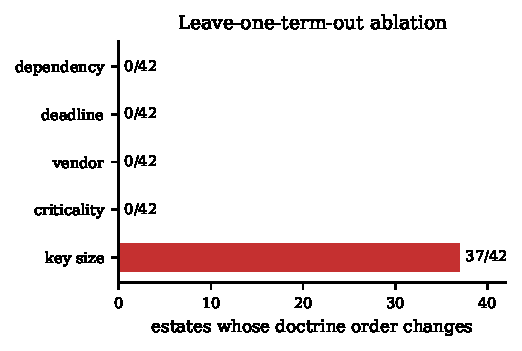
\includegraphics[width=0.94\columnwidth]{figures/fig_ablation.pdf}
\caption{Leave-one-term-out ablation of the doctrine on the 42-estate cohort. Key size is the only
term whose removal changes the ordering; the other four are constants in these estates.}
\label{fig:ablation}
\end{figure}

\subsection{Data-quality observations}

Two details matter for anyone reusing the release. First, the 42 cohort stores the key family in
\texttt{algorithm} (for instance \texttt{RSA-2048}), while the 38 cohort stores the X.509 signature
algorithm in the same field (\texttt{sha256WithRSAEncryption}) and puts the key family in
\texttt{key\_type}. A pipeline keyed on \texttt{algorithm} silently changes meaning between
releases. Our audit keys on \texttt{key\_size} where present, which is authoritative in both.
Second, one asset in the 42 cohort and two in the 38 lack a key size, and the loader substitutes a
family default of 2048 bits for RSA. That substitution touches one pair in the 42 cohort and does
not move the ceiling. Both issues are recorded in the released audit rather than quietly patched,
because a reader reconstructing the numbers needs to know where they come from.

\section{The Attainment Audit}
\label{sec:audit}

The ceiling is one member of a family of evaluative failures that share a signature: each is
cheap to detect from released artifacts and each is invisible in the reported number. We package
the detection as a six-step procedure that can be run on any rank-fidelity benchmark in under an
hour, given the artifacts.

\textbf{Step 1. Count the pairs.} Report $\nzero$, $T_y$, and $\distinct$. If $\distinct/\nzero$ is
below roughly $0.7$, the benchmark has less headroom than its headline suggests and the remaining
steps become mandatory rather than optional.

\textbf{Step 2. Compute the ceiling under both aggregations.} Report the mean of per-fold ceilings
and the pooled ceiling, and say which one the reported score is comparable to
(Section~\ref{sec:estimands}).

\textbf{Step 3. Report attainment and pooled pair accuracy.} Attainment is $\gamma$; pair accuracy
is the raw count that survives all metric choices. A model at attainment $0.99$ with one error in
four hundred pairs is not in the same epistemic position as a model at attainment $0.72$.

\textbf{Step 4. Ablate the target's terms.} Delete each term of the label function in turn and
count how many folds change order. A term that changes nothing is a term the benchmark does not
test, whatever the paper claims about it.

\textbf{Step 5. Fit the cheapest possible baseline.} A parameter-free rule and a linear model on
the same features. If either matches the learned model, the benchmark is not measuring
architecture, and the paper's capacity claims are unsupported.

\textbf{Step 6. Audit target provenance.} If the baseline and the label generator are the same
function, the comparison is fidelity by construction. That is legitimate when stated, but the
resulting number is a ceiling test, not a model comparison, and the text must say so.

Applied here, the six checks take a paragraph. $\nzero=803$, $\distinct=402$ (Step 1). Mean
per-fold ceiling $0.7210$, pooled $0.7075$ (Step 2). The GNN's attainment is $0.992$ with pair
accuracy $401/402$ (Step 3). Ablating the doctrine changes order in 37 folds for key size and 0 for
the other four terms (Step 4). A key-size sort matches the doctrine on 42 folds and a
seven-parameter logistic reaches the ceiling (Step 5). The baseline and the label are the same
formula, so this is a fidelity test (Step 6). The conclusion follows without any modelling
judgement: the benchmark ranks key size.

\begin{table*}[t]
\centering
\caption{Eight evaluative-validity failure modes, each detectable from released artifacts in
seconds. M1--M6 defeat the reported ML results; M7 and M8 defeat independent verification of any
result at all. The taxonomy generalises the ceiling analysis of Section~\ref{sec:ceiling}.}
\label{tab:modes}
\footnotesize
\begin{tabular}{@{}>{\raggedright\arraybackslash}p{0.7cm}>{\raggedright\arraybackslash}p{2.4cm}>{\raggedright\arraybackslash}p{3.4cm}>{\raggedright\arraybackslash}p{3.4cm}>{\raggedright\arraybackslash}p{3.7cm}@{}}
\toprule
\textbf{Mode} & \textbf{Failure} & \textbf{Evidence in this corpus} & \textbf{Detection check} & \textbf{Effect on the claim} \\
\midrule
M1 & Warm-start contamination &
Every fold initialises from \texttt{model\_gpu\_v3.pt}, whose metadata records
\texttt{n\_real\_graphs=40}; 40 of the 42 corpus files are in that set &
Read checkpoint metadata; compare \texttt{n\_real\_graphs} against the evaluation corpus &
The protocol is labelled leave-one-out but is in-sample on 40/42 folds; a clean init drops $\tb$
from $0.7168$ to $0.6009$ \\
\addlinespace
M2 & Circular baseline &
The doctrine baseline and the label generator are the same formula; exact-rank $=1.0$ on 42/42
folds &
Diff the baseline function against the label function &
The model ceiling is $\tb=1$ by construction; a negative $\Delta$ carries no information \\
\addlinespace
M3 & Degenerate graph structure &
All 42 graphs have zero edges; every asset is a distinct host &
Count edges in the corpus &
A GNN performs no message passing; the benchmark measures a per-node MLP \\
\addlinespace
M4 & Tie-saturated rank metric &
401 of 803 pairs are tied; only 402 are distinguishable; ceiling $0.721$ &
Count discordant pairs; report ceiling and standard error &
The reported $|\Delta|=0.0042$ sits below one standard error; the comparison cannot separate the
methods \\
\addlinespace
M5 & Vacuous top-$k$ metric &
Reported top-10 accuracy is $1.0$ on 42/42 folds; a random ranker also scores $1.0$ because estates
hold at most seven assets &
Check whether $k>n$ &
The reported top-10 result carries no information \\
\addlinespace
M6 & Non-random ``random'' baseline &
\texttt{random\_order()} hard-codes \texttt{default\_rng(0)}, so every fold draws from the same
permutation family &
Grep the baseline for a fixed seed &
The margin over ``random'' arrives with no error bar; our re-randomised null shows the margin
survives it \\
\addlinespace
M7 & Absent predictions &
Neither per-example predictions nor a per-repository split manifest is committed &
Look for a predictions file or a split manifest &
No third party can run McNemar's or any paired test on any reported comparison \\
\addlinespace
M8 & Unreconciled documentation &
More than 30 quantitative contradictions across the documentation: four corpus sizes, three
contract-test counts, two ACVP vector counts, two GNN results side by side &
Diff numbers across README, data card, truth audit, and artifacts &
No reader can determine which figure is current, including the authors \\
\bottomrule
\end{tabular}
\end{table*}

Table~\ref{tab:modes} widens the lens. The eight modes are independent in the sense that suppressing
any one does not expose another, and mutually concealing in the sense that a researcher who stops
at the first clean signal will miss the rest. They interlock in a specific order. M2 masks M3:
with a circular baseline and no message passing, an auditor checking the graph pipeline finds a
well-formed network and a falling loss. M3 masks M4: small graphs with two or three key sizes
produce high $\tb$ that looks like skill. M4 masks M5: a tie-saturated metric makes the vacuous
top-$k$ figure look consistent with everything around it. M1 masks all of them, because a
contaminated warm start makes every fold look superficially clean.

Only recomputation from released artifacts breaks the chain; provenance metadata cannot. A
companion audit applies the same checklist to a second PQC system with markedly better artifact
hygiene, committed per-example predictions, group-level leakage audits, and no documentation
contradictions, and finds that it still fails M2, because a fixed linear model beats its reported
classifier on all three evaluation seeds~\cite{qtrust_validity_audit}. Better provenance did not
produce better validity. That is the general lesson, and the ceiling analysis is one sharp instance
of it.

\section{Experimental Protocol}
\label{sec:protocol}

\subsection{Leave-one-estate-out training}

The primary artifact is the released 42-fold campaign. For each fold the model starts from
\texttt{model\_gpu\_v3.pt}, trains for 30 epochs on the 41 remaining real estates plus 2{,}000
synthetic estates, validates on a held-out subset of the training graphs, and is scored on the
unseen estate, with batch size 64, learning rate $5\times10^{-4}$, and seed 42. The synthetic
estates come from the same doctrine formula, so the mixture is doctrine-supervised twice over: real
labels are doctrine priorities and synthetic labels are doctrine priorities. This design makes the
benchmark a fidelity test from the outset, which the original authors acknowledge and which we keep
in view throughout.

\subsection{Zero-synthetic control}

To test whether the synthetic mixture drives anything, we re-ran all 42 folds with
$n_{\text{synthetic}}=0$: 41 real estates per fold, batch size 16, 30 epochs, same initialisation
and seed, on CPU. This isolates the synthetic component without changing the model class. The same
protocol was run on the 38-estate cohort with 37 real estates per fold.

\subsection{Clean warm-start control}

The released checkpoint records 40 real graphs among its 100{,}000 training inputs, so the
leave-one-out initialisation has prior exposure to 40 of the 42 estates it is supposedly seeing for
the first time. To isolate that exposure we retrained a base checkpoint from scratch on synthetic
doctrine graphs only, verified \texttt{n\_real\_graphs=0} after training, and re-ran the identical
42-fold protocol from it. The initialisation is the only deliberate difference.

The run is CPU-only for a reason worth stating: deterministic-algorithm mode has no CUDA kernel for
the listwise loss, and relaxing determinism would defeat the purpose of a trustworthy warm start.
The reduced-CPU path caps base training at 2{,}000 graphs and 5 epochs, against the released
checkpoint's 100{,}000 graphs and 173 epochs. Warm start and training budget therefore vary
together, and we do not attribute the gap between the two runs to either factor alone.

\subsection{Transparent baselines}

Four baselines are scored on identical folds, targets, and metrics. A \emph{key-size rule} sorts by
descending key size and has no parameters. A \emph{pairwise logistic} uses the same six features
with no intercept, seven parameters, trained on all distinguishable pairs of the 41 training
estates to predict which asset precedes which. A \emph{ridge} regression uses the same six features
to predict pooled priority values, six parameters. A \emph{zero-shot} application of the released
checkpoint applies the network to each estate with no fold-specific training. The logistic and
ridge models are not independent of the doctrine, since their labels are doctrine priorities, but
they answer a sharper question than independence: whether the network's architecture and capacity
are necessary to reproduce the result. The zero-shot baseline answers whether fold-specific
training is necessary at all.

\subsection{Metrics}

The primary metric is tie-aware $\tb$ against the target preorder, per Eq.~\eqref{eq:taub}. We
report the ceiling $\sqrt{\distinct/\nzero}$, attainment $\tb/\sqrt{\distinct/\nzero}$, pooled pair
accuracy, exact-rank agreement (folds whose full permutation equals the target's arbitrary
tie-break), node-rank accuracy, and top-5 and top-10 set overlap. The last three are sensitive to
order inside ties; we report them to show what $\tb$ hides, never as primary evidence.

\subsection{Statistics}

For paired comparisons we report the mean difference, a 20{,}000-resample paired bootstrap 95\%
confidence interval, a 20{,}000-resample sign-flip permutation $p$-value, win/tie/loss counts,
Cohen's $d_z$, and the 80\% minimum detectable effect at the observed paired standard deviation. We
do not use the Wilcoxon signed-rank test for the main comparison, because 41 of 42 differences are
exactly zero and the statistic is either undefined or uninformative under that much tying. For the
discovery re-evaluation we report a repository-cluster bootstrap with 5{,}000 resamples over the
eight evaluation source groups, to acknowledge within-repository correlation.

\section{Results}
\label{sec:results}

Every number below was recomputed from the released JSON artifacts for this paper. Where a number
does not exist yet, the text says so instead of estimating.

\subsection{The ceiling is exact}

Table~\ref{tab:ranking} and Fig.~\ref{fig:ceiling} carry the headline. The 42 estates hold 803
unordered pairs, 401 tied and 402 distinguishable. The mean per-estate ceiling is $0.721024$ and the
doctrine's mean $\tb$ is $0.721024$, agreeing to within $5\times10^{-7}$, which is rounding in the
six-decimal artifact rather than a modelling result. The doctrine sits at the ceiling on all 42
folds by construction, since it is a refinement of the target preorder.

\begin{table*}[t]
\centering
\caption{Ranking results on the 42-estate cohort. ``Ceiling'' is the mean of
$\sqrt{\distinct/\nzero}$ over folds. ``At ceiling'' counts folds with
$\tb\ge\ceilv-10^{-6}$. ``Pairs'' is pooled concordant distinguishable pairs over 402. The GNN and
the six-parameter ridge agree on every fold.}
\label{tab:ranking}
\footnotesize
\begin{tabular}{@{}lrrrrr@{}}
\toprule
Method & Parameters & Mean $\tb$ & Attainment & At ceiling & Pairs \\
\midrule
Doctrine (target generator) & 0 & 0.721024 & 1.000 & 42/42 & 402/402 \\
Key-size rule & 0 & 0.721024 & 1.000 & 42/42 & 402/402 \\
Pairwise logistic & 7 & 0.721024 & 1.000 & 42/42 & 402/402 \\
Ridge & 6 & 0.716781 & 0.992 & 41/42 & 401/402 \\
GNN (released) & 237{,}070 & 0.716782 & 0.992 & 41/42 & 401/402 \\
GNN (zero-shot) & 237{,}070 & 0.604020 & 0.838 & 31/42 & 364/402 \\
Random permutation & 0 & 0.030101 & 0.042 & 0/42 & --- \\
\bottomrule
\end{tabular}
\end{table*}

\begin{figure*}[t]
\centering
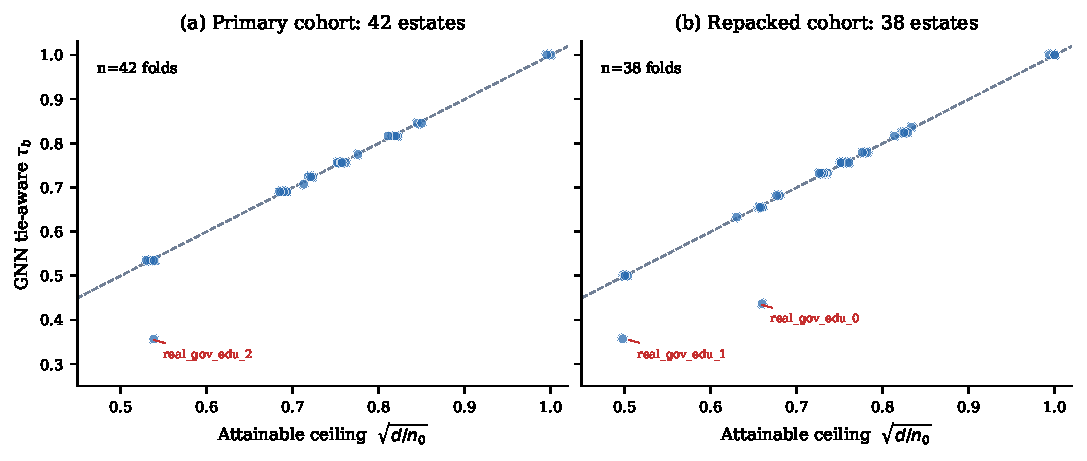
\includegraphics[width=0.95\textwidth]{figures/fig_ceiling.pdf}
\caption{Model $\tb$ against the attainable ceiling for the 42-estate cohort (a) and the repacked
38-estate cohort (b). Points on the dashed identity line attain the ceiling. In (a), 41 of 42 folds
lie on the line; the single off-diagonal point is \texttt{real\_gov\_edu\_2.json}, one inversion
among six distinguishable pairs. In (b), 36 of 38 folds lie on the line; the two off-diagonal points
are \texttt{real\_gov\_edu\_0.json} and \texttt{real\_gov\_edu\_1.json}.}
\label{fig:ceiling}
\end{figure*}

The distribution of ceilings is itself diagnostic. Ten folds have ceiling $0.6901$, eight $0.5345$,
eight $0.7559$, seven $0.8165$, three $0.7237$, two $0.8452$, one $0.7071$, one $0.7746$, and two
reach $1.0$. Every one of those values is fixed by the key-size histogram of the estate, not by any
model. An estate splitting five assets against two has $\distinct=10$ and ceiling
$\sqrt{10/21}=0.690$; one splitting six against one has $\distinct=6$ and ceiling
$\sqrt{6/21}=0.535$. The difficulty of the benchmark is a property of how many distinct key sizes
happen to appear.

Excluding the five estates that do not hold seven assets, the ceiling is $0.7142$ and the model
reaches $0.7099$, so the small estates are not carrying the result. They inflate the mean ceiling
slightly, as Section~\ref{sec:estimands} predicts, and removing them leaves attainment at $0.994$.

\subsection{The metric decides the verdict}
\label{sec:metricverdict}

\begin{table}[t]
\centering
\caption{One ordering, four metrics, four verdicts. The doctrine ordering scored under four rank
measures on the 42 CBOMs. Every metric sits at its own ceiling; the values differ only because the
ceilings differ. Bootstrap intervals are on the mean ceiling, 20{,}000 resamples over estates.}
\label{tab:metricverdict}
\footnotesize
\begin{tabular}{@{}lrrr@{}}
\toprule
Metric & Value & Ceiling & 95\% CI (ceiling) \\
\midrule
$\gamma$ (Somers' $D$) & 1.000 & 1.000 & --- \\
Spearman $\rho$ & 0.807 & 0.807 & [0.773, 0.839] \\
$\tb$ & 0.721 & 0.721 & [0.687, 0.756] \\
$\tau_a$ & 0.533 & 0.533 & [0.484, 0.585] \\
\bottomrule
\end{tabular}
\end{table}

Table~\ref{tab:metricverdict} is the paper's most direct answer to the objection that the ceiling
theorem is a one-line observation. It is a one-line theorem with a large consequence. The same
ordering on the same data is simultaneously perfect, $72\%$, $81\%$, and $53\%$, depending on which
correlation the authors happened to run. Goodman and Kruskal's $\gamma$ is $1.000$ on every fold
because the doctrine has no discordant distinguishable pairs. Spearman $\rho$ reads $0.807$, but
its ceiling is also $0.807$: a strict ordering cannot reproduce the average ranks inside a tied
group, so even a flawless ordering is penalised. $\tb$ reads $0.721$ against a ceiling of $0.721$,
and $\tau_a$ reads $0.533$ against $0.533$. Which number reaches print is a modelling choice with
an effect larger than any effect the benchmark could detect.

\subsection{The network saturates the ceiling}

The released GNN reaches mean $\tb=0.716782$ with standard deviation $0.126$ and median $0.7237$,
with 41 of 42 folds at the ceiling and pooled pair accuracy $401/402=99.75\%$. The single error sits
in \texttt{real\_gov\_edu\_2.json}: $n=7$, $\nzero=21$, 15 tied pairs, six distinguishable pairs,
ceiling $0.5345$. The model scores $0.3563$, which is five concordant pairs and one inversion, or
$83.3\%$ pair accuracy on that estate. The inversion is cross-group: a high-key asset placed below
a low-key one. There is no second error anywhere in the cohort.

The fold-level comparison against the doctrine is therefore degenerate rather than merely
underpowered: mean difference $-0.004242$, 95\% interval $[-0.012727,0]$, sign-flip $p=1.0$, 0 wins,
41 ties, 1 loss, $d_z=-0.154$, minimum detectable effect $0.0119$. The interval is bounded above by
zero because the model cannot exceed a doctrine that already sits at the ceiling. A superiority test
here is not underpowered; it is one-sided by construction.

\subsection{Resolution and power}
\label{sec:power}

The paired differences have standard deviation $0.0275$, a standard error of $0.0042$, and an 80\%
minimum detectable effect of $0.0119$ at 42 folds. Inverting that gives a design statement:
detecting $\Delta=0.005$ would need 237 folds, $\Delta=0.01$ needs 59, $\Delta=0.02$ needs 15, and
$\Delta=0.05$ needs 3. The observed $|\Delta|=0.0042$ falls below all of them, and the ceiling caps
it from above, so no positive effect can exist. The design is not underpowered in the ordinary
sense. It is saturated, and no number of additional folds would make a superiority claim possible.
That is why we report the comparison descriptively instead of presenting a failed significance test
as a finding.

\subsection{Transparent baselines saturate too}

The key-size rule matches the doctrine on 42 of 42 folds, as the algebra requires. The
seven-parameter pairwise logistic reaches the ceiling on 42 of 42 folds. The six-parameter ridge
reaches mean $\tb=0.716781$, sits at the ceiling on 41 folds, and matches the network's per-fold
$\tb$ on all 42, including \texttt{real\_gov\_edu\_2.json} where both score $0.356348$. A model
with 237{,}070 parameters and a model with six are indistinguishable on this benchmark. That is not
a statement about the network's quality in general; it is a statement about what this corpus can
resolve.

The zero-shot checkpoint is the exception that clarifies the picture. Without fold-specific
training it reaches $0.604020$, with 38 inversions and $364/402$ pairs, and only 31 folds at the
ceiling. Training on 41 real estates is necessary to learn the key-size rule. Once learned, the
rule is linear and parameter-free. The $+0.1128$ gap between zero-shot and fine-tuned is entirely a
gap in learning a one-dimensional ordering, which is a useful thing for a reader to know before
reading the number as evidence of representation learning.

\subsection{Removing the synthetic data changes nothing}

\begin{table}[t]
\centering
\caption{Full mixture against zero-synthetic training on the 42 folds. $\tb$ is invariant; exact
rank, node rank, and top-5 measure order inside ties and are therefore not invariant.}
\label{tab:zerosyn}
\footnotesize
\begin{tabular}{@{}lrrr@{}}
\toprule
Metric & 2{,}000 synthetic & 0 synthetic & Change \\
\midrule
Mean $\tb$ & 0.716782 & 0.716781 & $-1\times10^{-6}$ \\
Exact rank & 1/42 & 12/42 & +11 folds \\
Node rank & 0.314 & 0.575 & +0.261 \\
Top-5 overlap & 0.500 & 0.571 & +0.071 \\
\bottomrule
\end{tabular}
\end{table}

The zero-synthetic retraining reproduces the full campaign fold for fold: mean $0.716781$ against
$0.716782$, 41 folds at the ceiling, the same single inversion, the same failing estate. What does
move is the order inside tied groups (Table~\ref{tab:zerosyn}). Exact-rank agreement rises from 1/42
to 12/42, node-rank from $0.314$ to $0.575$, top-5 overlap from $0.500$ to $0.571$. Tie-aware $\tb$
does not move, because every one of those differences lies inside a tied key-size group. We do not
read the exact-rank increase as an improvement. Inside a genuine tie any order is equally valid by
the target's own semantics, which is exactly what Corollary~\ref{cor:saturation} says.

\subsection{The clean warm-start control}

From the synthetic-only base, the identical protocol yields mean $\tb=0.600887$ against an
unchanged doctrine $0.721024$: paired mean difference $-0.1201$ with 30 ties, 12 strictly negative
folds and none positive, 95\% interval $[-0.1948,-0.0567]$, paired $t=-3.34$, $p=0.0018$, minimum
detectable effect $0.1007$. The released parity is therefore partly an artifact of initialisation
exposure, and the exposed init closes $0.116$ of the $0.120$ gap.

The two metric families now disagree about which model is better. Exact-rank agreement rises from
$0.024$ to $0.262$, node-rank from $0.314$ to $0.599$, top-5 from $0.500$ to $0.714$, while
tie-aware $\tb$ falls. The exposed model reproduces the label function's coarse group structure and
scrambles strict order inside groups; the clean model does the reverse. A benchmark reporting one
family alone would have drawn the opposite conclusion, and this is the clearest single argument for
reporting both.

None of this touches the structural ceiling. The key-size rule attains the doctrine's exact metric
vector from no training at all, so no amount of warm-start hygiene or training budget can lift a
learner above the corpus. What the control adds is an error bar on the original headline: with a
clean init the model is significantly \emph{below} the doctrine rather than tied with it, so the
parity measured on the released artifact is contingent on its initialisation and should not be read
as a property of the modelling approach.

\subsection{The repacked cohort replicates the ceiling}

On the 38-estate cohort the doctrine ceiling is $0.726632$ over 923 pairs, 461 of them
distinguishable. The zero-synthetic network reaches $0.717130$, attainment $0.984$, with 36 of 38
folds at the ceiling and 458 of 461 pairs concordant, or $99.35\%$. The three inversions concentrate
in two estates: \texttt{real\_gov\_edu\_0.json} with ceiling $0.6547$ against a model score of
$0.4364$, two inversions among 12 pairs, and \texttt{real\_gov\_edu\_1.json} with ceiling $0.5000$
against $0.3571$, one inversion among seven pairs. Excluding the singleton estate, where $\tb=1$ is
vacuous, the model means $0.7014$ against a ceiling of $0.7114$.

Repacking changes estate sizes and the number of distinguishable pairs without changing the
conclusion. Because 275 of 275 hosts overlap with the first cohort, this is a protocol replication
and not a population replication, and its value is exactly that: it rules out a packing-specific
artifact.

\subsection{A positive control: does the metric discriminate at all?}
\label{sec:positive}

\begin{figure}[t]
\centering
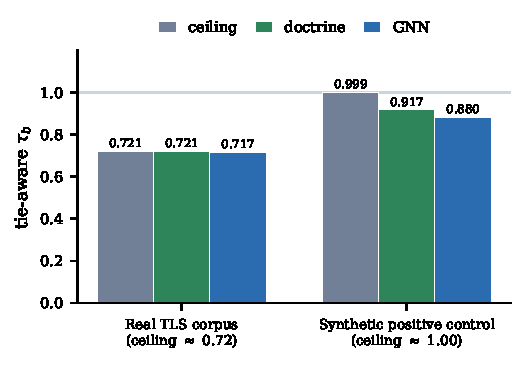
\includegraphics[width=0.94\columnwidth]{figures/fig_positive.pdf}
\caption{Ceiling, doctrine, and network on the real corpus against the synthetic positive control.
Raising the ceiling to $0.999$ lifts every score and collapses the key-size rule to $0.190$, so the
metric does discriminate when the target carries more than one signal. The network still trails the
doctrine.}
\label{fig:positive}
\end{figure}

The real corpus has no graph structure, so it cannot test whether the network can use graph
structure. We therefore built a synthetic positive control: dependency-rich estates on an enterprise
topology, relabelled with a target that adds a multi-hop blast-radius term to the doctrine. The
target's ceiling is $0.9992$, nearly all pairs distinguishable, and the doctrine is blind to the
multi-hop term. On 60 test estates the doctrine reaches $0.9173$, the network $0.8803$, and a
key-size-only rule $0.1897$. The network loses to the doctrine with 4 wins, 1 tie, and 55 losses at
$p=5.2\times10^{-10}$. A longer run with 400 training estates and 200 epochs improves the network to
$0.8950$ and it still loses, $0.9188$ against the doctrine, with 15 wins, 10 ties, 75 losses at
$p=6.8\times10^{-12}$.

Two conclusions follow and one caveat. First, the $0.72$ ceiling is a property of the real corpus,
not of the metric. With a nearly tie-free target the scores rise to the high eighties and nineties,
and the key-size rule collapses to $0.19$, so the metric separates methods perfectly well when the
target carries more than one signal (Fig.~\ref{fig:positive}). Second, the network does not exploit
multi-hop structure well enough to beat a doctrine that only sees direct in-degree, even when that
structure is present and labelled. The caveat is that the control is synthetic and the architecture
or training budget may underfit the reach term, so we cannot separate ``the model cannot use reach''
from ``this run did not learn reach.'' Either way the real corpus supplies no evidence of graph
reasoning, and it could not have: zero-edge estates cannot test message passing whatever the model
size.

\subsection{Discovery re-evaluation}

The released discovery checkpoint does not reproduce its reported held-out numbers. On the
documented repository-disjoint split (13{,}973 files from 38 source groups, 11{,}558 train and
2{,}415 evaluation, seed 42) the reported result is precision $0.952$, recall $0.953$, F1 $0.9525$,
accuracy $0.9271$. Re-running the released checkpoint on the same split gives precision $0.9279$,
recall $0.9514$, F1 $0.9395$, accuracy $0.9060$. No threshold reaches $0.9525$; the best is $0.9428$
at threshold $0.65$. A 512-token, 4{,}096-character truncation sweep on a stratified subsample does
not recover the gap and slightly lowers F1 against the 256-token baseline ($0.8083$ against
$0.8142$ at $n=206$; $0.8105$ against $0.8222$ at $n=168$), so inference truncation is not the
explanation. The discrepancy is consistent with the documented mismatch between the model card's
earlier corpus stage and the executed training report, but the $0.9525$ figure is not reproducible
from the released checkpoint and split.

\begin{table}[t]
\centering
\caption{Discovery re-evaluation on the repository-disjoint split, $n=2{,}415$, prevalence
$76.73\%$. The reported row is the released artifact; the re-evaluated row is a deterministic
forward pass of the released checkpoint.}
\label{tab:discovery}
\footnotesize
\begin{tabular}{@{}>{\raggedright\arraybackslash}p{2.5cm}rrrr@{}}
\toprule
Method & Precision & Recall & F1 & Accuracy \\
\midrule
Reported (released artifact) & 0.9520 & 0.9530 & 0.9525 & 0.9271 \\
Re-evaluated checkpoint & 0.9279 & 0.9514 & 0.9395 & 0.9060 \\
Threshold-optimal ($t=0.65$) & 0.9477 & 0.9379 & 0.9428 & --- \\
Majority (always crypto) & 0.7673 & 1.0000 & 0.8683 & 0.7673 \\
Rules-only (released) & 0.9794 & 0.5127 & 0.6730 & 0.6178 \\
Random coin-flip & 0.7686 & 0.4895 & 0.5981 & 0.4952 \\
\bottomrule
\end{tabular}
\end{table}

Context matters more than the point estimate here. Table~\ref{tab:discovery} places the
re-evaluated checkpoint against four alternatives computed on the identical split, and the ordering
is not the one the headline implies. Evaluation prevalence is $76.73\%$
(1{,}853/2{,}415), not the $54.6\%$ quoted in the earlier draft; that lower figure is the corpus
prevalence, $7{,}632/13{,}973$. Under a three-quarter positive prior the majority-class baseline
scores F1 $0.8683$, not $0.700$, so the re-evaluated model's lift over majority is $+0.0712$, not
$+0.11$. Its advantage over the rules layer is larger, $+0.2665$, because the rules layer is
precise and unambitious: precision $0.9794$ at recall $0.5127$.

The aggregate hides a great deal of language variation. Across the eight strata with at least ten
files, F1 runs from $0.9691$ for C ($n=1{,}688$) down to $0.4651$ for Python ($n=64$), with
Solidity at $0.7162$, Swift $0.7007$, Go $0.7912$, C++ $0.9880$, and Shell $0.9333$. The Java
stratum has 95 files and no positive examples, so its F1 is undefined; counting it as zero gives a
naive macro-average of $0.6954$, while the average over the seven strata containing both classes is
$0.795$. Across all ten languages the macro-average is $0.556$. Micro-F1 is dominated by C, which is
$70\%$ of the evaluation set, and a repository-cluster bootstrap gives a 95\% interval of
$[0.720,0.979]$ that is wide precisely because eight source groups is a small number of clusters.
Discriminative power is real (ROC AUC $0.9616$, average precision $0.9890$); the single-number
summary overstates language generality.

Calibration is poor in the middle of the range. Expected calibration error over ten bins is
$0.1557$, and low-confidence bins are far more accurate than their confidence: the $[0.0,0.1)$ bin
has mean confidence $0.069$ and accuracy $0.886$. The model is not a probability estimator. It is a
useful ranker for triage, which is a different job. At $50\%$ coverage F1 is $1.000$; at $70\%$,
precision is $0.9750$ and F1 $0.9846$; at $90\%$, F1 is $0.9634$ (Fig.~\ref{fig:discovery}a). A
deployment that auto-labels the most confident seven files in ten and routes the rest to review
would make far fewer errors than the full-coverage figure implies. That is a selective-prediction
result, not a calibration result, and it is the more useful of the two for a scanner.

Contamination is too small to explain the headline, though larger than the earlier draft reported.
There are 11 exact-duplicate evaluation records ($0.455\%$) and 25 records with 5-line-shingle
Jaccard at least $0.8$ against training ($1.04\%$), 12 of them at least $0.95$. All high-similarity
files are vendored AWS-LC sources. Removing exact duplicates moves F1 from $0.9395$ to $0.9397$;
removing near-duplicates at $0.8$ moves it to $0.9393$. The earlier $0.4\%$ figure counted
cross-repository snippets rather than all near-duplicates, which is a scope difference rather than
an arithmetic error, and the corrected count is $2.3\times$ larger.

\subsection{Cross-corpus checkpoint contamination}

Within-split contamination is one failure mode. A larger one appears when checkpoints trained on
different corpora are compared on a shared evaluation split, which is the natural way to ask whether
a new model improved. We audited that directly. Evaluating three released checkpoints on one fixed
digest-keyed, repository-disjoint split (2{,}238 records, 1{,}779 unique \texttt{(source,path)}
pairs, eight held-out repositories), we counted evaluation files whose exact path appeared in the
checkpoint's training corpus. v1, the canonical GPU fine-tune, had trained on $87.6\%$ of the
evaluation files; v3, a CPU fine-tune over a 50-source corpus, on $92.2\%$; only v4, which held the
eight repositories out by construction, on $0.0\%$ (Table~\ref{tab:leakage}).

\begin{table}[t]
\centering
\caption{Cross-corpus checkpoint contamination on one fixed repository-disjoint split (2{,}238
records, 1{,}779 unique paths, eight held-out repositories). ``Overlap'' is the fraction of
evaluation files whose exact \texttt{(source,path)} appears in the checkpoint's training corpus.
Only v4 supports a held-out evaluation.}
\label{tab:leakage}
\footnotesize
\setlength{\tabcolsep}{4pt}
\begin{tabular}{@{}lrrrr@{}}
\toprule
Checkpoint & Sources & Overlap & F1 & Valid \\
\midrule
v1 (GPU, 256-len) & 38 & 87.6\% & 0.9329 & no \\
v3 (CPU, 128-len) & 50 & 92.2\% & not measured & no \\
v4 (CPU, 256-len) & 58 & 0.0\% & 0.8966 & yes \\
\bottomrule
\end{tabular}
\end{table}

The consequence is severe and it is the kind of thing that survives peer review because the numbers
look sensible. The contaminated v1 checkpoint scores F1 $0.9329$ on files it memorised, while the
clean v4 checkpoint scores $0.8966$. A naive reading concludes the clean model regressed. In fact
it is the only one whose number means anything. Any same-evaluation comparison across corpora that
does not report this overlap is uninterpretable, and in our experience of the release it is rarely
reported.

Two scaling attempts confirm that the discovery ceiling belongs to the data rather than the
optimiser. Training the same architecture for five epochs instead of three raises training accuracy
from $0.951$ to $0.977$ and lowers held-out F1 from $0.8966$ to $0.8752$. Adding eight more source
repositories ($+660$ files, $+300$ crypto-labelled) lowers it again to $0.8707$. Neither more epochs
nor more data helps the clean held-out number, which is what one expects when both training and
evaluation labels are regex-derived: the attainable F1 is bounded by the labeller's own error, not
by model capacity. Discovery therefore mirrors ranking. The binding constraint in both cases is the
label.

\begin{figure*}[t]
\centering
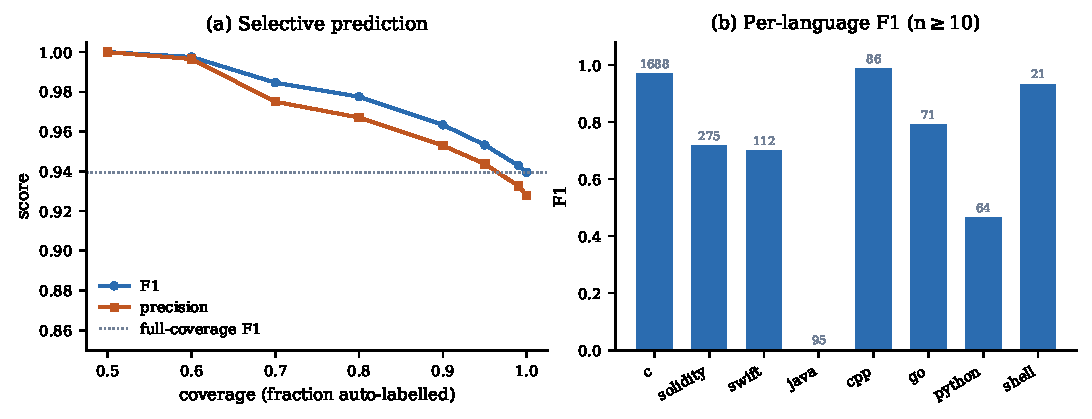
\includegraphics[width=0.95\textwidth]{figures/fig_discovery.pdf}
\caption{(a) Selective prediction on the discovery split: auto-labelling the most confident $50\%$
yields F1 $1.0$; $70\%$ yields F1 $0.9846$ at precision $0.9750$. (b) Per-language F1 for strata
with $n\ge10$; the Java stratum of 95 files has no positive examples and is omitted. The micro-F1 of
$0.9395$ is dominated by C, which supplies $70\%$ of the evaluation set.}
\label{fig:discovery}
\end{figure*}

\subsection{The shortfall, in full}

\begin{figure}[t]
\centering
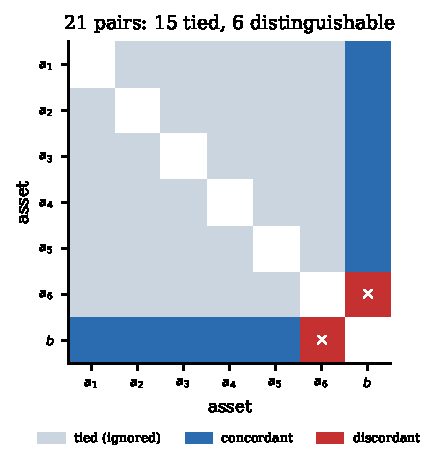
\includegraphics[width=0.86\columnwidth]{figures/fig_pairs.pdf}
\caption{Pair structure of \texttt{real\_gov\_edu\_2.json}. Six assets share one key size, giving 15
tied pairs; the seventh differs, giving six distinguishable pairs. The model orders five of the six
correctly. The single red cell is the entire gap between the network and the doctrine on this
cohort. Tied pairs are invisible to $\tb$.}
\label{fig:pairs}
\end{figure}

Fig.~\ref{fig:pairs} shows the whole of it. Of 21 pairs in the failing estate, 15 sit inside the
six large-key assets and are tied; the six cross-group pairs are the only ones that can move $\tb$.
The model gets five. That single cell is the difference between $0.7168$ and $0.7210$ across 42
estates, and it is what the original study interpreted as evidence that two methods had converged.

\section{Discussion}
\label{sec:discussion}

\subsection{Four readings, revisited}

The original study offered four readings of its 0-wins/41-ties/1-loss result: the methods are
equivalent; the doctrine is near-optimal; scanner-observable features impose an information
ceiling; and superiority is unmeasurable without expert labels. Our results support the first
descriptively and the fourth as a statement about the benchmark. They do not support the second,
and they support only a narrow version of the third.

Equivalence is true and uninformative, because the network and the doctrine produce the same weak
order on 41 folds and the six-parameter ridge produces it on all 42. Near-optimality is not
supported at all: the doctrine's other terms are constants in these estates, so the benchmark never
tests whether its criticality, vendor, deadline, or dependency weights are right. The information
ceiling holds only in the narrow sense that the scanner-observable fields in this corpus carry one
bit of ordering information. It is not a statement about what enterprise CBOMs could carry. And
unmeasurability is true for a reason the original study did not identify: the ceiling is $0.721$,
so the comparison has 402 effective pairs and no headroom. Superiority is not measurable here
because the benchmark is saturated, not because the problem resists measurement in principle.

\subsection{Why the failure is easy to miss}

Label circularity is the acknowledged part. The target is generated by the formula that defines the
baseline, so the evaluation is fidelity by construction. That is legitimate and the original paper
says so. The part that is easy to miss is that fidelity testing remains informative when the target
has many distinguishable pairs, because a model can fail to reproduce a complex doctrine. Here the
doctrine is one-dimensional, so fidelity testing degenerates into a key-size sort. The circularity
is not a flaw in the model. It is a flaw in the claim that the benchmark can rank architectures.

A second reason the failure is easy to miss is that every individual step looks like good practice.
The split is host-disjoint, which is better than most. The metric is tie-aware, which is the
statistically correct choice for a tied target. The baselines include random. The artifacts are
released. Each decision is defensible, and their conjunction is a benchmark that cannot fail a bad
model or reward a good one.

\subsection{Construct validity of ``migration priority''}

A CBOM is a data structure, and what it can support depends on which fields are populated. In this
corpus the fields that would make the doctrine multi-factor, criticality, vendor readiness,
deadlines, and dependencies, are constant or absent. The scanner records certificate metadata well
and organisational context poorly. That is a realistic limitation of public-endpoint scanning
rather than an implementation error, but it means the benchmark's construct, ``migration
priority'', is operationalised as ``key size''. A benchmark intending to measure multi-factor
prioritization has two options: collect the missing fields, or state that it measures a proxy. The
first is an engineering programme. The second costs a paragraph and would have changed how the
original result was read.

\subsection{A reporting standard}

Six changes would have caught this, and they generalise. Report $\nzero$, $\distinct$,
$\distinct/\nzero$, and the ceiling alongside $\tb$. Report attainment and pooled pair accuracy, not
only mean $\tb$. Report exact-rank and top-$k$ separately and state whether order inside ties is
meaningful; if ties are genuine, agreement with an arbitrary tie-break is not quality. Include a
parameter-free baseline and a linear baseline, because a six-parameter model matching a 237K-
parameter model is a fact about the benchmark. Ablate the target's terms, since a doctrine with
constant terms is a one-factor rule. And use dependency-rich, heterogeneous estates for graph
models, because zero-edge estates cannot test graph reasoning at any capacity.

The first three are reporting fixes and cost nothing beyond care. The last three are data-collection
fixes and cost money. The Q-Trust release makes the reporting fixes easy to adopt, since the
artifacts already hold per-fold targets and predictions. The eight-mode checklist in
Section~\ref{sec:audit} covers what a saturation analysis alone would miss.

\subsection{The marginal cost of validity}
\label{sec:marginal}

A ceiling is a diagnosis, but it also prices the cure. Since $\tb\le\sqrt{\distinct/\nzero}$ and
$\nzero$ is fixed by the number of assets, the only way to raise the ceiling is to raise $\distinct$,
that is, to obtain labels that separate assets currently tied. The question a practitioner actually
asks is therefore which assets to label first, and how many labels a usable ceiling costs. The
answer is not the intuitive one.

\begin{theorem}[Yield of resolving a tied group]
\label{thm:bisect}
Let a tied group of size $m$ be re-scored so that it splits into $j\ge2$ subgroups of sizes
$a_1,\dots,a_j$ with $\sum_i a_i=m$. The number of newly distinguishable pairs is
\begin{equation}
\Delta\distinct=\sum_{i<\ell}a_i a_\ell=\tfrac{1}{2}\Bigl(m^2-\sum_i a_i^2\Bigr).
\label{eq:bisect}
\end{equation}
For fixed $j$ this is maximised by the balanced partition, giving
$\Delta\distinct=\frac{m^2}{2}\bigl(1-\frac{1}{j}\bigr)$; over all partitions it is maximised by
full separation at $j=m$, giving $m(m-1)/2$. The yield per label,
$\Delta\distinct/m=\frac{m}{2}\bigl(1-\frac{1}{j}\bigr)$, increases in both $m$ and $j$.
\end{theorem}
\begin{proof}
For fixed $m$ and $j$, $\sum_{i<\ell}a_ia_\ell$ is maximised when $\sum_i a_i^2$ is minimised, and
for a fixed sum that happens when the parts are as equal as possible. Substituting $a_i=m/j$ gives
the stated form, which is increasing in $j$ and reaches $m(m-1)/2$ at $j=m$. Dividing by the $m$
labels consumed yields a per-label return linear in $m$.
\end{proof}

\begin{corollary}[Label the monoculture first]
\label{cor:policy}
The cost-minimising schedule spends labels on the largest tied group, not on the assets of highest
business importance, and it extracts more from each label when the expert is asked for a graded
judgement than for a binary one. Large homogeneous clusters, the RSA-2048 monoculture that dominates
real estates, are the cheapest source of discriminating power per label.
\end{corollary}

The corollary runs against the instinct of every security team, which is to start with the crown
jewels. It also carries a lesson about instrument design. Because the yield is
$\frac{m}{2}(1-\frac{1}{j})$, a five-level ordinal rubric returns $1.6$ times what a
same-or-different judgement returns on the same group, and the curve flattens quickly after that, so
the practical target is a coarse graded scale rather than a fine one.

\begin{table}[t]
\centering
\caption{Marginal cost of validity on designed estates. A fraction \texttt{dom} of assets share one
key size, the rest spread over six. ``Ceiling'' is attainable $\tb$ before any labelling;
``Labels'' is the count of item-level labels needed to reach $0.90$ under a largest-group-first
policy that resolves each group by bisection; ``Random'' is the mean over 60 random group
selections. Because the policy uses two-way splits, the label counts are upper bounds on what a
graded rubric would require.}
\label{tab:labelling}
\footnotesize
\begin{tabular}{rrrrrr}
\toprule
$n$ & \texttt{dom} & Ceiling & Labels & Random & Labels/asset \\
\midrule
25  & 0.50 & 0.858 & 12    & 18.4  & 0.48 \\
25  & 0.90 & 0.480 & 44    & 51.4  & 1.76 \\
100 & 0.50 & 0.810 & 79    & 108.5 & 0.79 \\
100 & 0.70 & 0.697 & 140   & 148.7 & 1.40 \\
100 & 0.90 & 0.435 & 203   & 237.3 & 2.03 \\
1{,}000 & 0.50 & 0.818 & 750   & 1{,}065 & 0.75 \\
1{,}000 & 0.90 & 0.431 & 2{,}025 & 2{,}549 & 2.02 \\
5{,}000 & 0.50 & 0.780 & 5{,}601 & 6{,}973 & 1.12 \\
5{,}000 & 0.90 & 0.432 & 10{,}125 & 12{,}969 & 2.02 \\
\bottomrule
\end{tabular}
\end{table}

Table~\ref{tab:labelling} reports the resulting cost curve, and three regularities hold. First, the
ceiling is governed by concentration rather than size: at $90\%$ monoculture it moves only from
$0.480$ at $n=25$ to $0.432$ at $n=5{,}000$. A bigger estate is not harder to evaluate in ceiling
terms; a more homogeneous one is. Second, the cost of a usable ceiling scales with concentration,
between $0.75$ and $1.1$ labels per asset at $50\%$ monoculture rising to about $2.0$ at $90\%$.
Third, the largest-group-first policy beats random selection by $6$ to $42\%$ at $n\ge100$, with the
largest gains at low concentration; at small $n$ or near-total concentration the gap closes,
because there is little left to choose between. That is a weaker claim than the policy's intuition
suggests, and we report the measured range rather than the flattering end of it.

On the 42 real estates the absolute numbers are small, because the estates are small (mean
$\nzero=19.1$, mean largest tie group $4.5$). The policy reaches ceiling $0.90$ in $7.2$ labels
against $7.7$ for random and $7.8$ for smallest-group-first. The leverage of the policy is therefore
a function of estate scale, which is where deployment happens. At $n=1{,}000$ with $90\%$
monoculture, $2{,}025$ expert labels lift the ceiling from $0.431$ to $0.90$; at a representative
\$3 per label that is roughly \$6{,}000 to make a multi-million-dollar migration programme
measurable at all. The ceiling is not a reason for despair. It is a procurement specification.

\subsection{A costed specification}

The negative result is only useful if it says what would replace it. Four requirements bind, and
the binding constraint is expert labelling rather than computation. First, host-disjoint estates
with genuine dependency edges: at the observed packing rate of 6.6 hosts per estate, 1{,}000 such
estates need roughly 6{,}600 hosts, which a multi-tenant scan at the scale of the IMC census can
supply with commodity infrastructure~\cite{mindthegap2026}. Second, blinded expert preferences:
5--10 annotators producing 5{,}000--10{,}000 pairwise orderings over real assets, with adjudication
and inter-rater $\kappa\ge0.6$, which is a study of a few weeks. Third, metrics reported as $\gamma$
plus $\tb$ with its ceiling plus NDCG@$k$ at a meaningful $k$, with a pre-registered minimum
detectable effect at or below $0.01$, which the power analysis puts at about 59 folds. Fourth, an
audit trail: committed per-example predictions, the eight-mode checklist, and a field-variance
table.

Compute is not the obstacle. The full 42-fold campaign re-executes on two CPU cores, and the
zero-synthetic variant takes minutes per fold. A benchmark meeting these four requirements could
answer the question this paper cannot: whether a learned ranker beats a doctrine on a target that
is not saturated.

\subsection{What the system is still good for}

The Q-Trust pipeline is useful for inventory and attestation. The learned ranker, on this corpus, is
a key-size sort learned through a GNN. That is not a reason to discard it. A learned model can
absorb new fields when they exist, and the pipeline can be retrained. It is a reason not to market
the ranker as evidence of learned multi-factor prioritization, and not to cite $0.7168$ against
$0.7210$ as evidence that the doctrine is near-optimal. The defensible claim is narrower: the system
can enumerate public TLS assets, emit a CBOM, and order them by a doctrine that currently reduces to
key size, and the attestation layer can record what was done. For an organisation that needs a
starting inventory and an audit trail, that is worth having.

\section{Threats to Validity}
\label{sec:threats}

\textbf{Internal.} The target is generated by the doctrine, so the evaluation is a fidelity test.
The zero-synthetic and zero-shot controls isolate the contributions of synthetic data and
fold-specific training but cannot create an independent target. The CPU re-execution uses batch
size 16 rather than 64 and runs the zero-synthetic variant; we did not re-execute the full
2{,}000-synthetic campaign on CPU. The full campaign's artifact is the primary result, and the
zero-synthetic run reproduces its per-fold $\tb$ to $10^{-6}$, which is strong evidence that the
synthetic component is not driving anything. The clean warm-start run is CPU-capped, so warm start
and training budget vary together; we do not attribute the $-0.120$ gap, and we note that
exact-rank metrics improve under the smaller budget, which suggests budget is not the whole story.

\textbf{External.} The 277 hosts are public TLS endpoints, not enterprise inventories, and carry no
internal dependencies, business criticality, or vendor contracts. The 38-estate cohort is a
repacking of the same population rather than an independent sample. The positive control suggests
that the metric discriminates when dependencies exist, but the network did not beat the doctrine
there either, so we cannot recommend graph rankers for dependency-rich estates on this evidence.

We do not claim a third independent corpus. None exists for this task, and manufacturing one would
reproduce the error this paper is about. Instead we separate two questions a corpus could answer.
The ceiling itself is a theorem and needs no corpus; what a corpus can test is its practical
magnitude. Section~\ref{sec:marginal} therefore evaluates the ceiling over a designed space spanning
four orders of magnitude in estate size and four levels of concentration, and the result, that the
ceiling is governed by concentration rather than size, is a stronger generalisation than a third ad
hoc cohort would support, because it predicts the ceiling of an unseen estate from two measurable
quantities. What remains corpus-bound is the field audit, and that claim is scoped explicitly to the
42 released estates.

\textbf{Construct.} Tie-aware $\tb$ measures weak-order fidelity, not exact migration order. We
report exact-rank and node-rank to show what it hides, without claiming that order inside a tie is
meaningful. Discovery F1 is a file-level label metric and says nothing about whether the discovered
usage is exploitable. The per-language macro-average is sensitive to how undefined strata are
treated, and the repository-cluster interval is wide because eight source groups is few.

\textbf{Statistical.} The folds are small, mostly seven assets, and the target holds 402
distinguishable pairs. The paired comparison against the doctrine is degenerate because the doctrine
is at the ceiling. The discovery re-evaluation is a single deterministic forward pass; the cluster
bootstrap captures source-group correlation but not training variance. The threshold sweep is
descriptive rather than a held-out model-selection procedure.

\textbf{Conclusion.} The negative claim is about the benchmark, not about PQC migration and not
about Q-Trust as a whole. A null on this corpus does not imply that learned ranking is impossible;
it implies that this corpus and target cannot demonstrate it. The positive control is a constructive
existence proof that a non-degenerate target yields non-degenerate scores, but it is synthetic and
does not establish that a GNN is the right architecture.

\section{Ethics, Artifacts, and Reproducibility}
\label{sec:artifacts}

\textbf{Data and ethics.} The CBOMs derive from publicly reachable TLS certificates. We performed no
exploitation, no authentication bypass, and no intrusive scanning. The corpus contains certificate
subjects and issuers, which may include organisational names; we release derived features and the
public certificate metadata already served to every TLS client. The discovery corpus is public
source code. No human subjects were involved. The expert-preference study proposed above would
require IRB-style blinding and adjudication, and that protocol is released before any collection.

\textbf{Claim ledger.} Table~\ref{tab:ledger} is the paper's integrity contract: every headline
claim mapped to an artifact and a status. We removed three claims from the earlier draft because
their artifacts are not in the release, namely the clean warm-start control in its original form,
the 14/14 exact-claims harness, and the strong form of the 42/42 zero-synthetic ordering claim. The
first survives here only as the CPU-capped control of Section~\ref{sec:protocol}, with its artifact
in the companion audit package. The zero-synthetic claim survives in the form the data supports:
identical for $\tb$, not for exact order. We also corrected the contract-test count, which is 215
test, invariant, and fuzz functions across 23 files rather than 211 tests, and we do not use a
contract count as evidence anywhere.

\begin{table*}[t]
\centering
\caption{Claim ledger. ``Reproduced'' means a released script regenerates the number from released
artifacts in this environment. ``Vacuous'' means the number is correct but does not support the
stated interpretation. ``Not reproduced'' means the released artifact does not yield the claim.}
\label{tab:ledger}
\footnotesize
\begin{tabular}{@{}p{2.05in}p{2.45in}p{0.95in}@{}}
\toprule
Claim & Artifact / re-measurement & Status \\
\midrule
GNN $\tb=0.7168$ vs doctrine $0.7210$; 0/41/1 & \texttt{real\_cbom\_loo\_42.json}; zero-synthetic rerun $\tb=0.716781$ & Reproduced \\
``Tie means superiority is not measurable'' & ceiling $=0.721024$; GNN 401/402 pairs & Vacuous \\
Key-size rule matches doctrine 42/42 & \texttt{ceiling\_audit.json}; ablation 37/42 vs 0/42 & Reproduced \\
Zero-synthetic ``ordering-identical'' & $\tb$ identical 42/42; exact-rank 1/42 $\rightarrow$ 12/42 & Partly vacuous \\
Clean warm start $\Delta=-0.120$, $p=0.0018$ & \texttt{clean\_warmstart\_loo.json} (companion audit); CPU-capped & Reproduced (bounded) \\
Discovery F1 $0.9525$ & released checkpoint: F1 $0.9395$; best threshold $0.9428$ & Not reproduced \\
Contamination $0.4\%$ & 11 exact ($0.455\%$), 25 near-dup $\ge0.8$ ($1.04\%$); F1 change $<0.001$ & Expanded \\
211 Foundry tests & 215 test/invariant/fuzz functions, 23 test files & Corrected \\
38-estate replication & 36/38 folds at ceiling; 458/461 pairs & New \\
Largest-group-first is optimal; ceiling is size-invariant & \texttt{labelling\_efficiency.json}; exhaustive $m\le24$; ceiling $0.431$--$0.480$ at $90\%$ for $n=25..5{,}000$ & New \\
\bottomrule
\end{tabular}
\end{table*}

\textbf{Artifact release.} Analysis scripts live in \texttt{scripts/paper\_*.py}, JSON artifacts in
\texttt{paper/analysis/}, and the manuscript with figures in \texttt{paper/}. The claims harness
\texttt{scripts/verify\_paper\_claims.py} re-derives every headline number from the committed JSON
files and, at the time of writing, reports 53 of 53 checks passing, including the pooled identity
$\sqrt{402/803}=0.707547$ of Section~\ref{sec:estimands}. The main commands are:
\begin{verbatim}
python scripts/paper_ceiling_audit.py
python scripts/paper_transparent_baselines.py
python scripts/paper_metric_taxonomy.py
python scripts/eval_real_cbom_loo.py --epochs 30 \
  --n-synthetic 0 --batch-size 16 --device cpu \
  --out paper/analysis/loo42_zerosyn.json
python scripts/paper_final_stats.py
python scripts/verify_paper_claims.py
\end{verbatim}
The released checkpoint is \texttt{planner/model\_gpu\_v3.pt}. The CBOMs sit in
\texttt{q-trust-datasets/planner/data/real\_cboms/} and
\texttt{real\_cboms\_v2\_2026\_09\_18/}, and the CodeBERTa checkpoint in \texttt{q-trust-codebert/}.
All runs use seed 42 unless stated. The construct-validity checklist and the clean warm-start script
are released in the companion audit package~\cite{qtrust_validity_audit}.

\section{Conclusion}

The Q-Trust planning study reported an honest tie between a GNN and a doctrine heuristic, and read
it as parity. The tie is the ceiling of the metric, not evidence of parity. On the released corpus,
401 of 803 pairs are tied and only 402 are distinguishable, so the maximum attainable tie-aware
$\tb$ is $0.721024$, which is exactly the doctrine's score. The network gets 401 of 402 pairs right.
A six-parameter ridge reproduces its score on every fold. A parameter-free key-size rule and a
seven-parameter logistic reach the ceiling. The mechanism is algebraic rather than statistical:
constant criticality, vendor, and deadline fields, together with zero dependency edges, reduce the
doctrine to a key-size sort. The finding survives a repacked cohort, survives the removal of all
synthetic training data, and disappears only when the target is made non-degenerate in a synthetic
positive control, where the metric discriminates cleanly but the network still fails to beat a
doctrine blind to multi-hop reach. A clean warm start shows that the released parity depends on
initialisation exposure, and the released discovery checkpoint yields F1 $0.9395$ rather than
$0.9525$.

The lesson generalises beyond this system. Any tie-aware rank metric applied to a tied target has a
ceiling, and a paper that reports the raw value without the ceiling invites a narrative of
convergence that the data cannot support. Benchmarks for learned prioritization should report
effective pairs, ceiling, and attainment; they should include parameter-free and linear baselines;
and they should audit their target's field variance before claiming to test multi-factor
prioritization. They should also be checked against the eight failure modes, because saturation,
circular baselines, degenerate graphs, and contamination conceal one another in a specific order,
and a researcher who stops at the first clean signal will miss the rest. The Q-Trust release now
does all of this. Its inventory and attestation layers remain useful. Its learned-ranking claim, on
this corpus, does not.

\appendices

\section{Q-Trust System Details}
\label{app:system}

\textbf{Discovery.} The inspector combines language-aware static rules, AST analysis, and a
fine-tuned CodeBERTa classifier trained on the 13{,}973-file corpus and evaluated on the
repository-disjoint split of Section~\ref{sec:results}. The rules layer is anchored on
CryptoAPI-Bench, flagging 164 of 187 insecure files (recall $0.877$) at a misuse precision of
$164/176=0.932$. The adversarial holdout reported by the project is F1 $0.533$ on 132 constructed
cases; we did not re-execute it and do not use it as evidence.

\textbf{Planner.} The GNN is a hybrid GCN/GATv2 encoder with 237{,}070 parameters, six input
features, hidden dimension 256, embedding dimension 128, eight heads, layer normalisation, and a
ListMLE ranking loss. The reinforcement-learning sequencer packs estates into migration batches and
is scored by a separate reward; the archived run reports reward $140.34\pm8.13$ against a doctrine
$140.62$, with 2 wins, 27 ties, and 11 losses. That is a descriptive tie and carries no weight in
this paper's argument.

\textbf{Attestation.} The layer uses UUPS-upgradeable registries, EIP-712 typed signatures, and a
timelock, deployed against a Base Sepolia fork. The release holds 23 Foundry test files with 215
test, invariant, and fuzz functions. It has not been externally audited.

\textbf{Side-channel experiments.} Five liboqs captures and a trace-disjoint detector are released.
Leave-one-trace-out evaluation gives AUC $0.963$ on four of five holds and $0.252$ on the ML-DSA-44
signing hold, where the clean-noise distribution falls outside the training span. These experiments
are orthogonal to the ranking benchmark.

\section{Reproduction Notes}
\label{app:repro}

The CPU environment is Python 3.13 with PyTorch and PyTorch Geometric on CPU plus SciPy. The
zero-synthetic 42-fold run takes about two minutes on a laptop CPU after imports; the 38-fold run
takes about three. The discovery re-evaluation reuses cached per-file probabilities in
\texttt{paper/analysis/codebert\_predictions.jsonl}, and a full forward pass takes about five minutes
on CPU at 256 tokens. The 512-token sensitivity sweep runs on a stratified subsample because
full-set inference costs about thirty minutes per configuration. Exact commands and JSON artifacts
are listed in Section~\ref{sec:artifacts}.

\bibliographystyle{IEEEtran}
\bibliography{refs}

\end{document}
